
\documentclass[11pt,letterpaper]{article}

% ---------------------------------------------------------
% Paquetes
% ---------------------------------------------------------

\usepackage[utf8]{inputenc}
\usepackage[T1]{fontenc}
\usepackage[spanish]{babel}
\usepackage{graphicx}
\usepackage{geometry}
\usepackage{amsmath}
\usepackage{listings}
\usepackage{xcolor}
\usepackage{float}
\usepackage[hidelinks]{hyperref}

\geometry{letterpaper, margin=2.1cm}

% ---------------------------------------------------------
% Configuracion de codigo
% ---------------------------------------------------------

\lstset{
    language=Python,
    basicstyle=\ttfamily\footnotesize,
    keywordstyle=\color{blue},
    commentstyle=\color{gray},
    stringstyle=\color{red!60!black},
    numbers=left,
    numberstyle=\tiny,
    frame=single,
    breaklines=true,
    showstringspaces=false,
    columns=fullflexible
}

% ---------------------------------------------------------
% Datos
% ---------------------------------------------------------

\title{Taller 5: Filtrado de Imágenes Digitales}

\author{
Camilo Eduardo Muñoz Albornoz\\
Procesamiento Digital de Imágenes\\
Universidad Tecnológica de Pereira
}

\date{}

\begin{document}

\maketitle

\begin{center}

\textbf{Código fuente en GitHub}\\[0.2cm]

\textbf{Repositorio: }
\href
{https://github.com/CamiloMunozAL/ProcDImagenes/tree/main/taller5}
{\textcolor{blue}{\underline{\texttt{Carpeta del Taller 5 en GitHub}}}}

\vspace{0.2cm}

\textbf{Cuaderno Python: }
\href
{https://github.com/CamiloMunozAL/ProcDImagenes/blob/main/taller5/taller5.ipynb}
{\textcolor{blue}{\underline{\texttt{taller5.ipynb}}}}

\end{center}

% =========================================================
\begin{abstract}

En este taller se estudiaron diferentes técnicas de filtrado
espacial aplicadas a imágenes digitales en escala de grises.
Se implementaron filtros paso bajo de promedio, media y
mediana, así como filtros paso alto para destacar bordes
y variaciones de intensidad.

Los algoritmos fueron desarrollados en Python utilizando
ciclos anidados, con apoyo de NumPy, OpenCV y Matplotlib.
Se utilizó una fotografía de un paisaje para observar
y comparar los efectos producidos por diferentes máscaras.

Finalmente, se evaluó la aplicación de un filtro de mediana
antes de un filtro paso alto, con el propósito de observar
cómo el suavizado previo influye en la identificación
de bordes y detalles de la imagen.

\end{abstract}

% =========================================================
\section{Objetivos}

Los objetivos del taller fueron:

\begin{enumerate}

    \item Desarrollar una función basada en ciclos que permita
    aplicar filtros paso bajo de promedio a una imagen,
    recibiendo como argumentos la imagen y una máscara.
    Observar los resultados obtenidos con tres máscaras:
    promedio uniforme $3\times3$, promedio uniforme
    $5\times5$ y promedio ponderado $3\times3$.

    \item Desarrollar una función basada en ciclos que permita
    aplicar filtros paso bajo de media de $3\times3$ y
    $5\times5$ a una imagen en escala de grises, recibiendo
    como entrada la imagen y obteniendo como salida
    la imagen filtrada.

    \item Desarrollar una función basada en ciclos para aplicar
    filtros paso bajo de mediana de $3\times3$ y $5\times5$
    a una imagen en escala de grises, observando los
    resultados obtenidos.

    \item Desarrollar una función basada en ciclos que permita
    aplicar filtros paso alto mediante máscaras de
    $3\times3$ y $5\times5$ a una imagen en escala de
    grises, analizando el efecto producido sobre
    los bordes y detalles.

    \item Aplicar primero un filtro de mediana a la imagen
    en escala de grises y posteriormente un filtro paso alto.
    Comparar este resultado con la aplicación directa
    del filtro paso alto sobre la imagen original,
    observando las diferencias en los bordes
    y detalles resaltados.

\end{enumerate}

% =========================================================
\section{Fundamentos teóricos}

\subsection{Filtrado de imágenes digitales}

El filtrado de imágenes digitales consiste en aplicar
operaciones matemáticas sobre los píxeles de una imagen
para modificar determinadas características.

Entre sus principales aplicaciones se encuentran
la reducción de ruido, el suavizado, el realce de
detalles y la detección de bordes.

El filtrado puede realizarse en el dominio espacial
o en el dominio de la frecuencia.

En este taller se trabajó principalmente con
\textbf{filtrado espacial}, donde las operaciones se
realizan directamente sobre los valores de los píxeles
y sus vecinos.

\subsection{Máscaras y operaciones de vecindad}

Una máscara o núcleo es una matriz pequeña que se
desplaza sobre la imagen y permite calcular un nuevo
valor para cada píxel.

Por ejemplo, una máscara de $3\times3$ considera
el píxel central y los ocho píxeles que lo rodean.

Su estructura general es:

\[
W =
\begin{bmatrix}
w_1 & w_2 & w_3\\
w_4 & w_5 & w_6\\
w_7 & w_8 & w_9
\end{bmatrix}
\]

En un filtrado lineal, cada valor de la máscara
se multiplica por el píxel correspondiente
de la vecindad y posteriormente se suman
los resultados.

Para una máscara simétrica de $3\times3$:

\[
g(x,y)=
\sum_{i=-1}^{1}
\sum_{j=-1}^{1}
f(x+i,y+j)w(i,j)
\]

Donde:

\begin{itemize}

    \item $f(x,y)$ representa la imagen original.
    \item $w(i,j)$ representa los coeficientes de la máscara.
    \item $g(x,y)$ representa el valor obtenido
    después del filtrado.

\end{itemize}

El tamaño y los coeficientes de la máscara
determinan cómo se modifica la imagen.

\subsection{Filtros paso bajo}

Los filtros paso bajo atenúan las variaciones rápidas
de intensidad entre píxeles vecinos.

Estas variaciones suelen estar relacionadas
con bordes, texturas finas y determinados tipos
de ruido.

Por esta razón, su aplicación produce un efecto
de suavizado o desenfoque.

Entre los filtros paso bajo estudiados se encuentran:

\begin{itemize}

    \item Filtro de promedio.
    \item Filtro de media.
    \item Filtro de mediana.

\end{itemize}

\subsubsection{Filtro de promedio}

El filtro de promedio reemplaza cada píxel por
una combinación de las intensidades de sus vecinos,
utilizando los coeficientes de una máscara.

Una máscara uniforme de $3\times3$ es:

\[
W_1=\frac{1}{9}
\begin{bmatrix}
1&1&1\\
1&1&1\\
1&1&1
\end{bmatrix}
\]

En este caso todos los píxeles tienen
la misma importancia.

También se pueden utilizar máscaras ponderadas,
que asignan pesos diferentes a los píxeles.

Por ejemplo:

\[
W_3=\frac{1}{16}
\begin{bmatrix}
1&2&1\\
2&4&2\\
1&2&1
\end{bmatrix}
\]

En esta máscara, el píxel central tiene
mayor peso que los demás.

\subsubsection{Filtro de media}

El filtro de media calcula el promedio aritmético
de las intensidades de una vecindad.

Su expresión general es:

\[
g(x,y)=\frac{1}{N}
\sum_{k=1}^{N}P_k
\]

Donde $N$ corresponde al número de píxeles
de la ventana.

Para una ventana de $3\times3$:

\[
N=9
\]

Mientras que para una ventana de $5\times5$:

\[
N=25
\]

El filtro de media es equivalente a un filtro
de promedio con coeficientes uniformes.

\subsubsection{Filtro de mediana}

El filtro de mediana es un filtro no lineal.

A diferencia del filtro de media, no calcula
un promedio aritmético, sino que ordena
las intensidades de la vecindad y selecciona
el valor central de la lista ordenada.

Por ejemplo:

\[
P=\{100,102,101,103,255,99,100,102,101\}
\]

Después de ordenar:

\[
P=\{99,100,100,101,101,102,102,103,255\}
\]

La mediana es:

\[
\operatorname{Mediana}(P)=101
\]

Este procedimiento resulta especialmente útil
para reducir ruido impulsivo, como el ruido
de sal y pimienta, sin modificar tanto
algunos contornos importantes.

\subsection{Filtros paso alto}

Los filtros paso alto destacan las variaciones
rápidas de intensidad presentes en una imagen.

Estas variaciones corresponden principalmente
a bordes, detalles finos y texturas.

Una máscara paso alto de $3\times3$ es:

\[
W=
\begin{bmatrix}
-1&-1&-1\\
-1&8&-1\\
-1&-1&-1
\end{bmatrix}
\]

Una característica importante es que
la suma de sus coeficientes es cero:

\[
8-8=0
\]

Esto significa que una región completamente
uniforme produce una respuesta igual a cero.

En cambio, cuando existen diferencias importantes
entre el píxel central y sus vecinos,
la respuesta puede tener una magnitud elevada.

Los resultados pueden ser positivos o negativos,
por lo que es necesario utilizar tipos de datos
que permitan representar ambos signos.

Para visualizar la magnitud de las respuestas
se puede utilizar el valor absoluto:

\[
g_{\text{visual}}(x,y)=|g(x,y)|
\]

Si se desea representar el resultado en
una imagen de 8 bits, los valores deben
ajustarse al intervalo de 0 a 255.

\subsection{Tratamiento de los bordes}

Cuando una máscara se aproxima al límite
de una imagen, parte de su vecindad puede
quedar por fuera de las dimensiones disponibles.

Este problema se conoce como
\textbf{problema del contorno}.

En las implementaciones de los filtros paso bajo
se decidió procesar solamente los píxeles
que permiten utilizar una ventana completa,
conservando los bordes originales.

En el filtro paso alto se inicializó la imagen
de salida con ceros, por lo que las posiciones
exteriores que no fueron procesadas
permanecieron en cero.

% =========================================================
\section{Desarrollo y resultados}

\subsection{Preparación de la imagen}

Para todos los ejercicios se utilizó una fotografía
de un paisaje que contiene montañas, árboles,
vegetación, cielo y un lago con reflejos.

Esta imagen permite observar el comportamiento
de los filtros sobre regiones uniformes,
bordes y zonas con diferentes texturas.

Se cargó directamente en escala de grises
utilizando OpenCV.

\begin{lstlisting}
import cv2
import numpy as np
import matplotlib.pyplot as plt

imagen = cv2.imread(
    'images/paisaje.png',
    cv2.IMREAD_GRAYSCALE
)

print("Tamano de la imagen:", imagen.shape)
\end{lstlisting}

La función \texttt{cv2.IMREAD\_GRAYSCALE}
permite cargar la fotografía utilizando
un único canal de intensidad.

Los píxeles se representan normalmente
mediante valores enteros entre 0 y 255.

% =========================================================
\subsection{Punto 1: Filtros paso bajo de promedio}

\subsubsection*{Objetivo}

Implementar mediante ciclos una función
que reciba una imagen y una máscara,
y devuelva la imagen filtrada.
Aplicar tres máscaras de promedio y analizar
sus efectos sobre la imagen.

\subsubsection*{Implementación}

Se definieron las tres máscaras solicitadas:

\[
W_1=\frac{1}{9}
\begin{bmatrix}
1&1&1\\
1&1&1\\
1&1&1
\end{bmatrix}
\]

\[
W_2=\frac{1}{25}
\begin{bmatrix}
1&1&1&1&1\\
1&1&1&1&1\\
1&1&1&1&1\\
1&1&1&1&1\\
1&1&1&1&1
\end{bmatrix}
\]

\[
W_3=\frac{1}{16}
\begin{bmatrix}
1&2&1\\
2&4&2\\
1&2&1
\end{bmatrix}
\]

En Python:

\begin{lstlisting}
mascara1 = np.ones((3, 3)) / 9

mascara2 = np.ones((5, 5)) / 25

mascara3 = np.array([
    [1, 2, 1],
    [2, 4, 2],
    [1, 2, 1]
]) / 16
\end{lstlisting}

Posteriormente se desarrolló una función
que recorre la imagen y la máscara
mediante cuatro ciclos anidados.

\begin{lstlisting}
def filtro_promedio(imagen, mascara):

    # Dimensiones de la imagen
    filas_imagen, columnas_imagen = imagen.shape

    # Dimensiones de la mascara
    filas_mascara, columnas_mascara = mascara.shape

    # Extension de la mascara
    extension_fila = filas_mascara // 2
    extension_columna = columnas_mascara // 2

    # Copia de la imagen original
    imagen_filtrada = imagen.astype(
        np.float64
    ).copy()

    # Recorrer la imagen
    for fila_imagen in range(
        extension_fila,
        filas_imagen - extension_fila
    ):
        for columna_imagen in range(
            extension_columna,
            columnas_imagen - extension_columna
        ):

            suma = 0

            # Recorrer la mascara
            for fila_mascara in range(filas_mascara):
                for columna_mascara in range(columnas_mascara):

                    pixel = imagen[
                        fila_imagen + fila_mascara
                        - extension_fila,

                        columna_imagen + columna_mascara
                        - extension_columna
                    ]

                    peso = mascara[
                        fila_mascara,
                        columna_mascara
                    ]

                    suma += pixel * peso

            imagen_filtrada[
                fila_imagen,
                columna_imagen
            ] = suma

    return np.clip(
        imagen_filtrada, 0, 255
    ).astype(np.uint8)
\end{lstlisting}

Los dos primeros ciclos recorren las posiciones
de la imagen y los dos últimos recorren
los elementos de la máscara.

Cada píxel se multiplica por su peso
correspondiente y los resultados se suman
para obtener la nueva intensidad.

Se utilizó una imagen de salida independiente
para evitar que los píxeles ya filtrados
modificaran los siguientes cálculos.

\subsubsection*{Aplicación}

\begin{lstlisting}
imagen_filtrada1 = filtro_promedio(
    imagen, mascara1
)

imagen_filtrada2 = filtro_promedio(
    imagen, mascara2
)

imagen_filtrada3 = filtro_promedio(
    imagen, mascara3
)
\end{lstlisting}

Los resultados se presentan en la
Figura~\ref{fig:promedio}.

\begin{figure}[H]
    \centering
    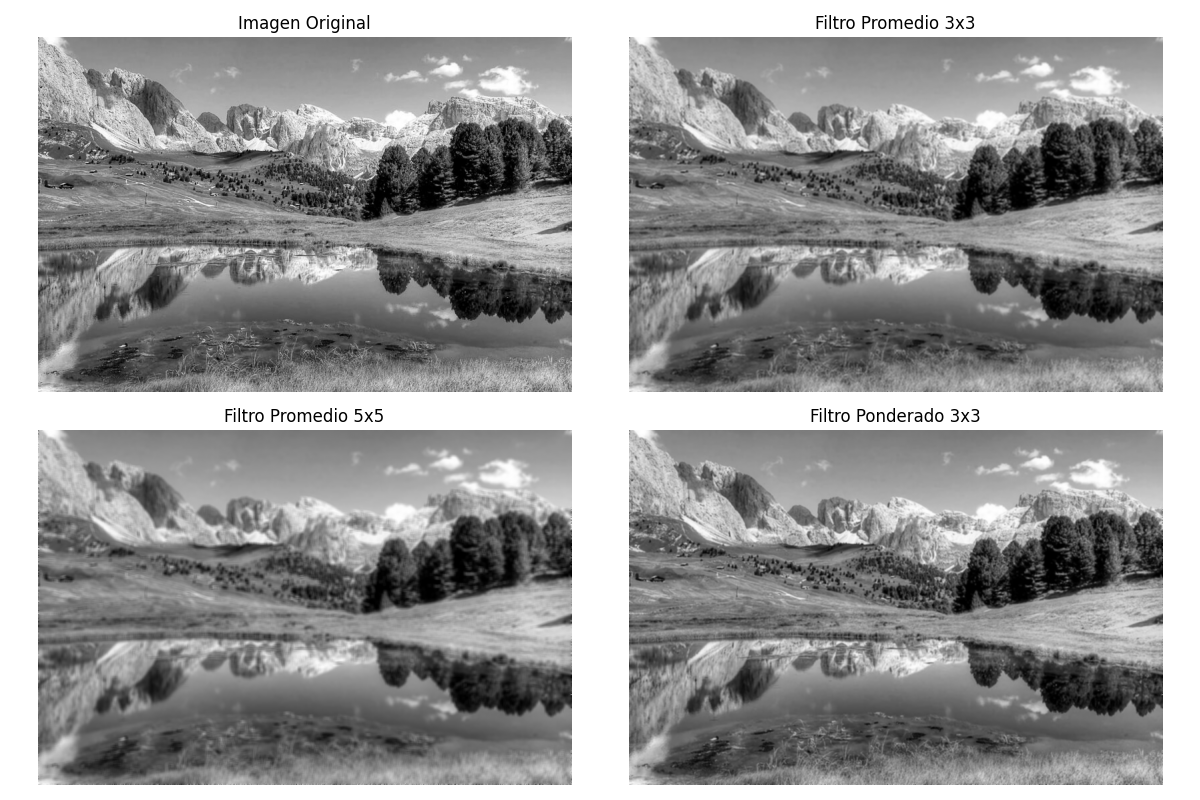
\includegraphics[width=\textwidth]
    {../results/resultado_filtro_promedio.png}
    \caption{Comparación de la imagen original con
    los filtros de promedio uniforme y ponderado.}
    \label{fig:promedio}
\end{figure}

\subsubsection*{Análisis de resultados}

Al comparar los resultados, se observa que
la máscara ponderada de $3\times3$ produce
el menor suavizado, conservando mejor
los detalles y bordes de las montañas,
los árboles y sus reflejos en el agua.

Por otra parte, la máscara uniforme de
$3\times3$ genera un suavizado mayor,
haciendo que los bordes de los árboles
y las montañas pierdan algo más de definición.

Finalmente, la máscara de $5\times5$
produce el desenfoque más evidente,
con una mayor pérdida de detalles.

Estas diferencias se deben tanto al tamaño
de la máscara como a la distribución
de sus coeficientes.

En la máscara ponderada, el píxel central
tiene mayor importancia, permitiendo
conservar mejor algunas características
de la imagen original.

En conclusión, los filtros paso bajo
reducen las variaciones de intensidad
entre píxeles vecinos, produciendo
un efecto de suavizado.

Sin embargo, también pueden provocar
una pérdida de detalles y definición
de los bordes.

En este caso, el filtro ponderado
de $3\times3$ ofreció el mejor equilibrio
visual entre suavizado y conservación
de detalles.

% =========================================================
\subsection{Punto 2: Filtros paso bajo de media}

\subsubsection*{Objetivo}

Desarrollar mediante ciclos una función
que permita aplicar filtros de media
de $3\times3$ y $5\times5$ a una imagen
en escala de grises.

\subsubsection*{Implementación}

En este punto se calculó directamente
el promedio aritmético de los píxeles
de cada vecindad.

Para una ventana cuadrada de tamaño $n$,
la operación es:

\[
g(x,y)=\frac{1}{n^2}
\sum_{i=-r}^{r}
\sum_{j=-r}^{r}
f(x+i,y+j)
\]

Donde:

\[
r=\left\lfloor\frac{n}{2}\right\rfloor
\]

La función desarrollada fue:

\begin{lstlisting}
def filtro_media(imagen, tamano):

    if tamano % 2 == 0 or tamano < 1:
        raise ValueError(
            "El tamano debe ser impar y mayor que 0"
        )

    # Dimensiones de la imagen
    filas_imagen, columnas_imagen = imagen.shape

    # Extension de la ventana
    extension = tamano // 2

    # Copia de la imagen original
    imagen_filtrada = imagen.astype(
        np.float64
    ).copy()

    # Recorrer cada pixel
    for fila_imagen in range(
        extension,
        filas_imagen - extension
    ):
        for columna_imagen in range(
            extension,
            columnas_imagen - extension
        ):

            suma = 0

            # Recorrer la vecindad
            for i in range(
                -extension,
                extension + 1
            ):
                for j in range(
                    -extension,
                    extension + 1
                ):

                    pixel = int(imagen[
                        fila_imagen + i,
                        columna_imagen + j
                    ])

                    suma += pixel

            # Calcular la media
            imagen_filtrada[
                fila_imagen,
                columna_imagen
            ] = suma / (tamano * tamano)

    return np.clip(
        imagen_filtrada, 0, 255
    ).astype(np.uint8)
\end{lstlisting}

A diferencia del punto anterior,
en este procedimiento no es necesario
multiplicar cada píxel por un coeficiente
de una máscara.

Simplemente se suman las intensidades
y se dividen entre el número de píxeles.

Además, se utilizó \texttt{int()}
al obtener cada píxel para evitar
desbordamientos durante la acumulación
de valores \texttt{uint8}.

\subsubsection*{Aplicación}

\begin{lstlisting}
imagen_media3 = filtro_media(imagen, 3)

imagen_media5 = filtro_media(imagen, 5)
\end{lstlisting}

El resultado se observa en la
Figura~\ref{fig:media}.

\begin{figure}[H]
    \centering
    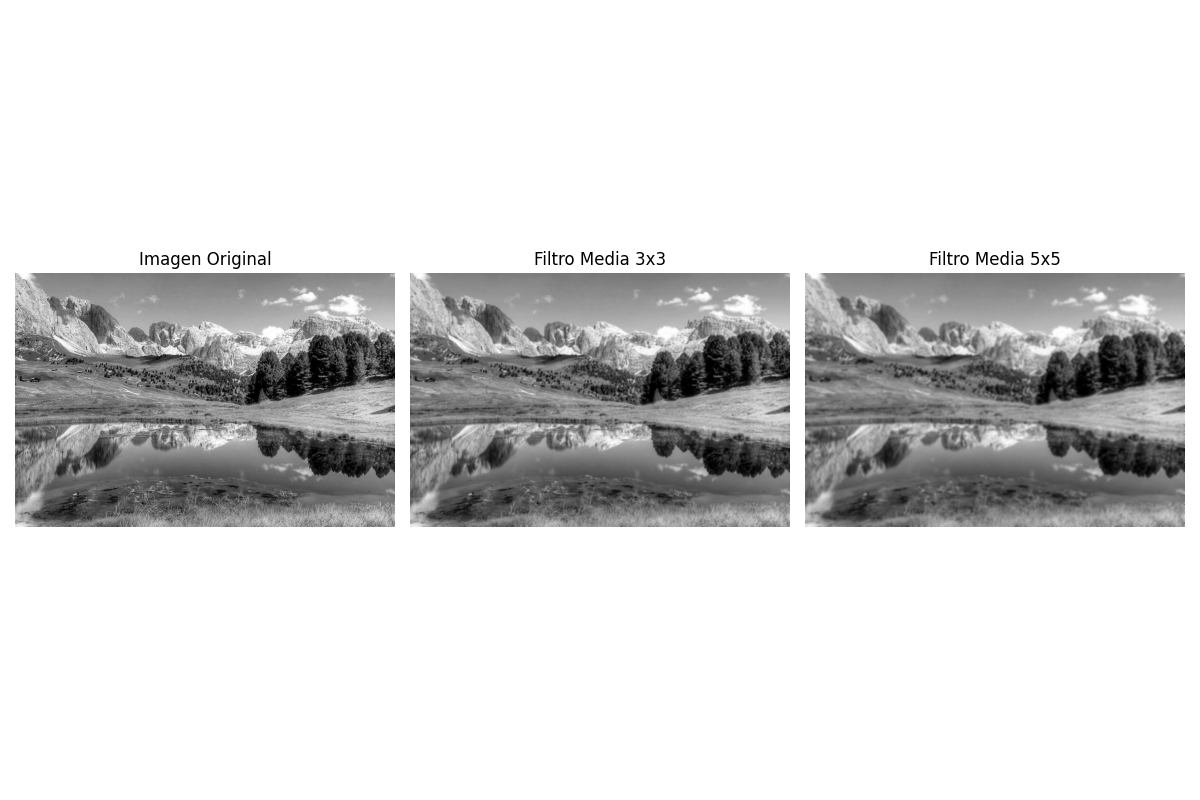
\includegraphics[width=\textwidth]
    {../results/resultado_filtro_media.png}
    \caption{Comparación de la imagen original
    con filtros de media de $3\times3$ y $5\times5$.}
    \label{fig:media}
\end{figure}

\subsubsection*{Análisis de resultados}

Al observar las imágenes, se evidencia
que el filtro de media $3\times3$
produce un suavizado ligero,
conservando gran parte de los detalles
de las montañas, los árboles y sus
reflejos en el agua.

Por otro lado, el filtro de media
$5\times5$ genera un desenfoque mayor,
haciendo que los bordes de las montañas,
los árboles y algunos detalles de la
vegetación pierdan más definición.

En conclusión, los filtros de media
permiten suavizar una imagen
al reducir las variaciones de intensidad
entre píxeles vecinos.

Se observa que, al aumentar el tamaño
de la ventana, el suavizado es mayor,
pero también se pierde más información
de los detalles y bordes.

% =========================================================
\subsection{Punto 3: Filtros paso bajo de mediana}

\subsubsection*{Objetivo}

Implementar mediante ciclos filtros
de mediana de $3\times3$ y $5\times5$
y observar su efecto sobre una imagen
en escala de grises.

\subsubsection*{Implementación}

El filtro de mediana obtiene los valores
de cada vecindad, los ordena de menor
a mayor y selecciona el valor central.

Para una ventana de $3\times3$ se
ordenan nueve valores y se selecciona
el quinto elemento.

Para una ventana de $5\times5$ se
ordenan 25 valores y se selecciona
el elemento número 13.

Debido a que Python utiliza índices
desde cero, las posiciones corresponden
a 4 y 12 respectivamente.

La función desarrollada fue:

\begin{lstlisting}
def filtro_mediana(imagen, tamano):

    if tamano % 2 == 0 or tamano < 1:
        raise ValueError(
            "El tamano de la mascara debe ser impar"
        )

    # Dimensiones de la imagen
    filas_imagen, columnas_imagen = imagen.shape

    # Extension de la ventana
    extension = tamano // 2

    # Copia de la imagen original
    imagen_filtrada = imagen.copy()

    # Recorrer cada pixel
    for fila_imagen in range(
        extension,
        filas_imagen - extension
    ):
        for columna_imagen in range(
            extension,
            columnas_imagen - extension
        ):

            # Extraer vecinos
            vecinos = []

            for i in range(
                -extension,
                extension + 1
            ):
                for j in range(
                    -extension,
                    extension + 1
                ):

                    pixel = int(imagen[
                        fila_imagen + i,
                        columna_imagen + j
                    ])

                    vecinos.append(pixel)

            # Ordenar los vecinos
            vecinos.sort()

            # Obtener la mediana
            mediana = vecinos[
                len(vecinos) // 2
            ]

            imagen_filtrada[
                fila_imagen,
                columna_imagen
            ] = mediana

    return imagen_filtrada
\end{lstlisting}

La lista \texttt{vecinos} almacena
las intensidades de cada ventana.

Posteriormente, el método \texttt{sort()}
ordena los valores y se obtiene
el elemento central.

De esta manera, el nuevo valor
del píxel corresponde a una intensidad
existente dentro de su vecindad.

\subsubsection*{Aplicación}

\begin{lstlisting}
imagen_mediana3 = filtro_mediana(imagen, 3)

imagen_mediana5 = filtro_mediana(imagen, 5)
\end{lstlisting}

Los resultados se muestran en la
Figura~\ref{fig:mediana}.

\begin{figure}[H]
    \centering
    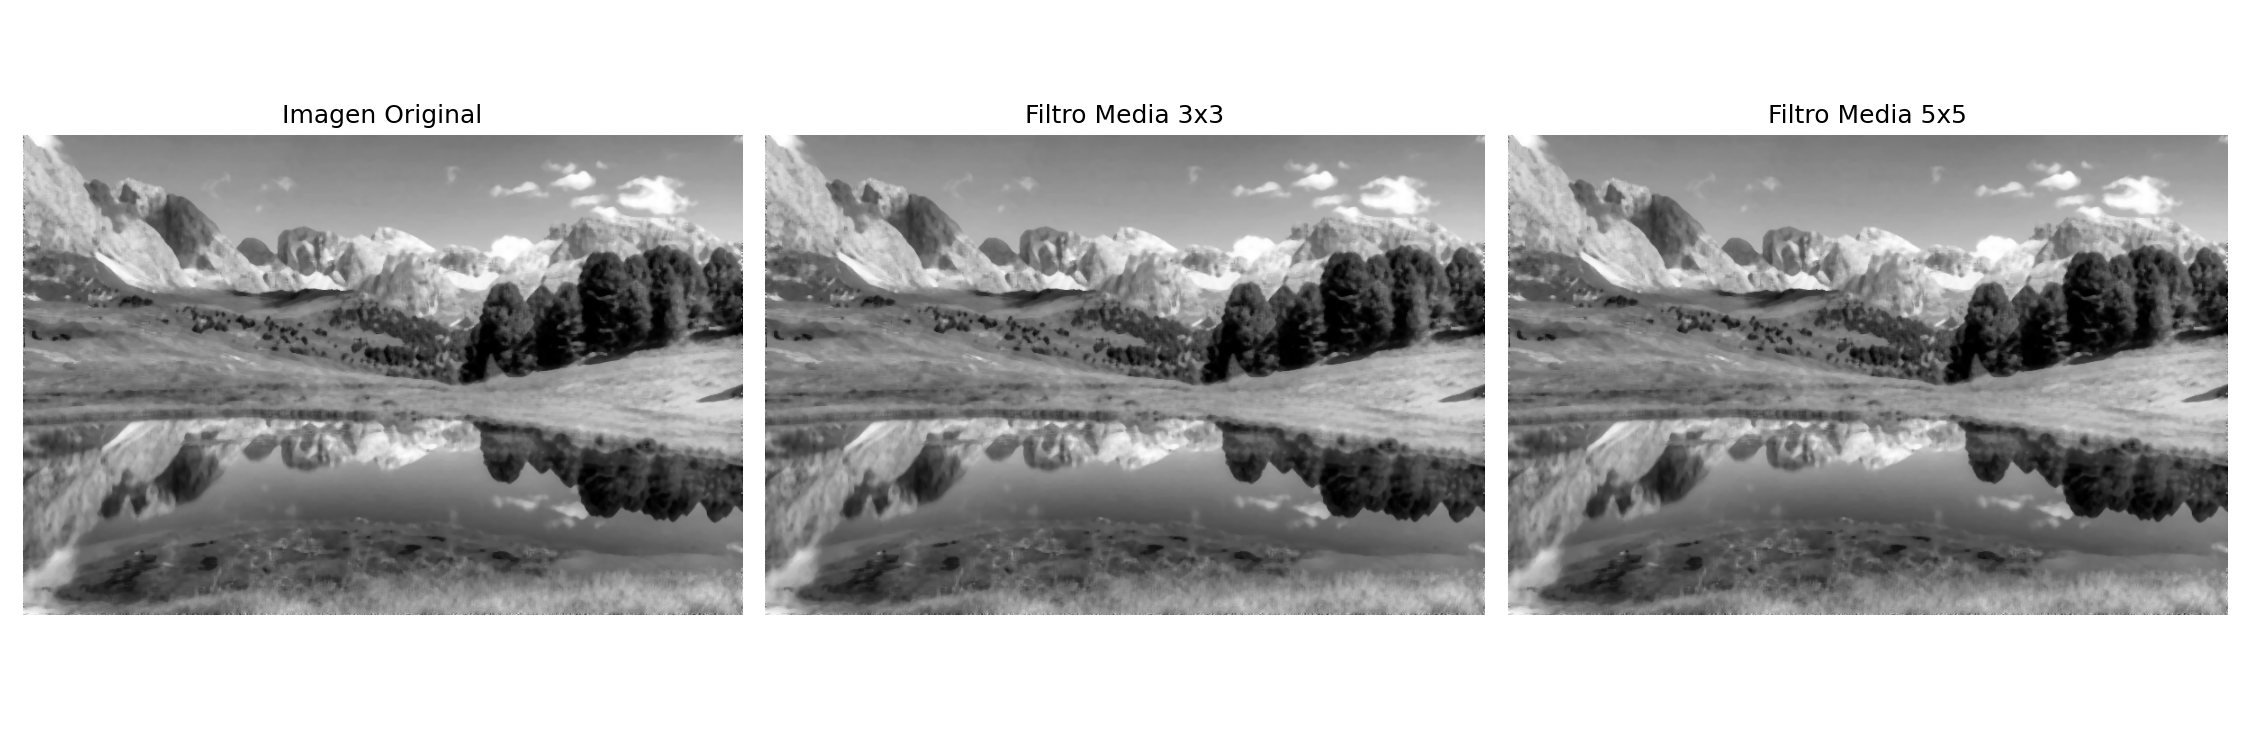
\includegraphics[width=\textwidth]
    {../results/resultado_filtro_mediana.png}
    \caption{Aplicación de filtros de mediana
    de $3\times3$ y $5\times5$.}
    \label{fig:mediana}
\end{figure}

\subsubsection*{Análisis de resultados}

Al observar los resultados, se evidencia
que el filtro de mediana $3\times3$
produce cambios leves en la imagen,
conservando gran parte de los detalles
y bordes de las montañas, los árboles
y sus reflejos en el agua.

Por otra parte, el filtro de mediana
$5\times5$ genera un suavizado mayor,
eliminando algunos detalles pequeños
de la vegetación y las texturas,
pero manteniendo relativamente bien
los contornos principales de los objetos.

Las diferencias respecto a la imagen
original no son muy pronunciadas,
debido a que la fotografía no presenta
una cantidad evidente de ruido impulsivo.

En conclusión, el filtro de mediana
permite reducir valores de intensidad
aislados y conservar relativamente bien
los bordes.

Al aumentar el tamaño de la ventana
se eliminan más detalles pequeños,
por lo que es importante seleccionar
el tamaño según las características
de la imagen.

% =========================================================
\subsection{Punto 4: Filtros paso alto}

\subsubsection*{Objetivo}

Desarrollar una función basada en ciclos
que permita aplicar filtros paso alto
mediante máscaras de $3\times3$
y $5\times5$, observando el realce
de cambios de intensidad y bordes.

\subsubsection*{Implementación}

Para el filtro paso alto $3\times3$
se utilizó la máscara:

\[
W_1=
\begin{bmatrix}
-1&-1&-1\\
-1&8&-1\\
-1&-1&-1
\end{bmatrix}
\]

Para la máscara $5\times5$ se asignó
un valor de $-1$ a las 24 posiciones
periféricas y un valor de 24 al centro:

\[
W_2=
\begin{bmatrix}
-1&-1&-1&-1&-1\\
-1&-1&-1&-1&-1\\
-1&-1&24&-1&-1\\
-1&-1&-1&-1&-1\\
-1&-1&-1&-1&-1
\end{bmatrix}
\]

Ambas máscaras tienen una suma
de coeficientes igual a cero.

Su implementación en Python fue:

\begin{lstlisting}
mascara_alto3 = np.array([
    [-1, -1, -1],
    [-1,  8, -1],
    [-1, -1, -1]
])

mascara_alto5 = -np.ones((5, 5))

mascara_alto5[2, 2] = 24
\end{lstlisting}

Posteriormente se construyó
la función para aplicar las máscaras
mediante ciclos anidados.

\begin{lstlisting}
def filtro_paso_alto(imagen, mascara):

    # Dimensiones de la imagen
    filas_imagen, columnas_imagen = imagen.shape

    # Dimensiones de la mascara
    filas_mascara, columnas_mascara = mascara.shape

    # Extension de la mascara
    extension_fila = filas_mascara // 2
    extension_columna = columnas_mascara // 2

    # Imagen de salida en float64
    imagen_filtrada = np.zeros_like(
        imagen,
        dtype=np.float64
    )

    # Recorrer cada pixel
    for fila_imagen in range(
        extension_fila,
        filas_imagen - extension_fila
    ):
        for columna_imagen in range(
            extension_columna,
            columnas_imagen - extension_columna
        ):

            suma = 0

            # Recorrer la mascara
            for fila_mascara in range(filas_mascara):
                for columna_mascara in range(columnas_mascara):

                    pixel = float(imagen[
                        fila_imagen + fila_mascara
                        - extension_fila,

                        columna_imagen + columna_mascara
                        - extension_columna
                    ])

                    peso = mascara[
                        fila_mascara,
                        columna_mascara
                    ]

                    suma += pixel * peso

            imagen_filtrada[
                fila_imagen,
                columna_imagen
            ] = suma

    return imagen_filtrada
\end{lstlisting}

La imagen de salida se inicializó
con valores cero y tipo
\texttt{float64}, debido a que
los filtros paso alto pueden generar
respuestas negativas y superiores a 255.

A diferencia de los filtros paso bajo
anteriores, no se convierten
inmediatamente los resultados a
\texttt{uint8}, con el fin de conservar
la información de los cálculos.

\subsubsection*{Aplicación}

\begin{lstlisting}
imagen_alto3 = filtro_paso_alto(
    imagen, mascara_alto3
)

imagen_alto5 = filtro_paso_alto(
    imagen, mascara_alto5
)

# Magnitud absoluta de las respuestas
imagen_alto3_visual = np.clip(
    np.abs(imagen_alto3),
    0,
    255
).astype(np.uint8)

imagen_alto5_visual = np.clip(
    np.abs(imagen_alto5),
    0,
    255
).astype(np.uint8)
\end{lstlisting}

Los resultados se presentan en la
Figura~\ref{fig:pasoalto}.

\begin{figure}[H]
    \centering
    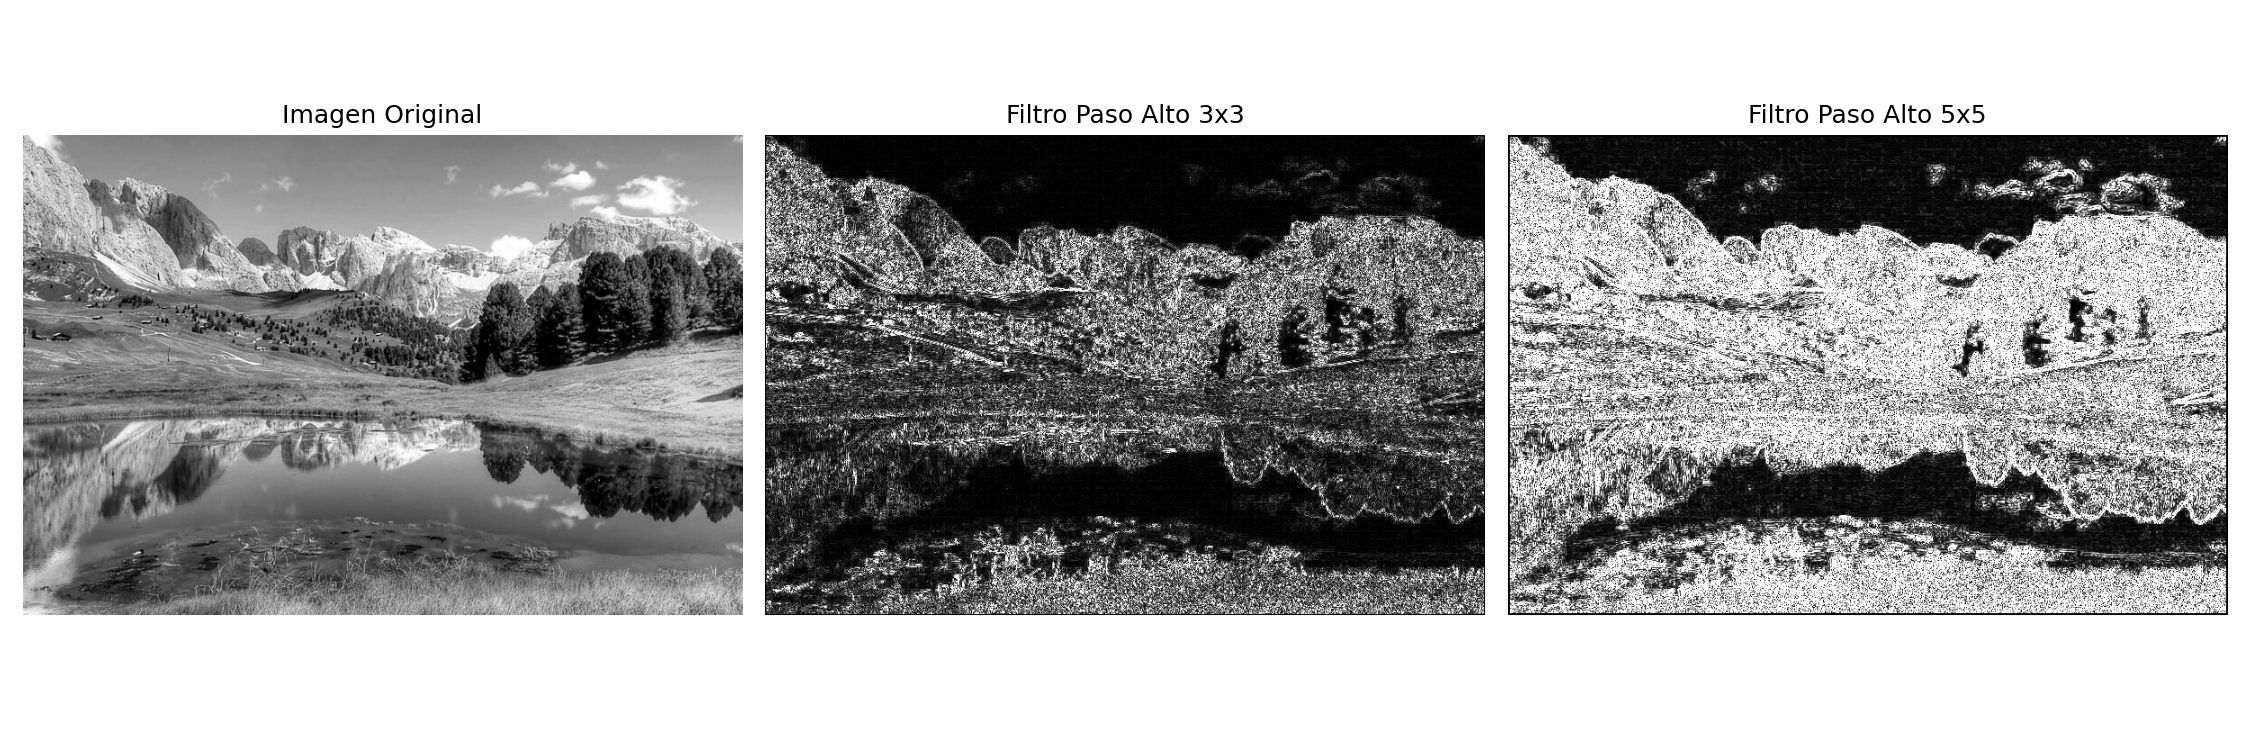
\includegraphics[width=\textwidth]
    {../results/resultado_filtro_paso_alto.png}
    \caption{Comparación de la imagen original
    con filtros paso alto de $3\times3$ y $5\times5$.}
    \label{fig:pasoalto}
\end{figure}

\subsubsection*{Análisis de resultados}

Al observar las imágenes, se evidencia
que el filtro paso alto $3\times3$
destaca los bordes de las montañas,
los árboles y algunas texturas
de la vegetación.

Por otra parte, las regiones más uniformes,
como el cielo y algunas zonas del agua,
aparecen oscuras debido a que presentan
pocas variaciones de intensidad.

En el filtro paso alto $5\times5$
se observa una respuesta mucho más intensa,
especialmente en las montañas,
los árboles y el pasto.

Esto se debe a que la máscara
considera una vecindad mayor y utiliza
coeficientes que pueden generar valores
de mayor magnitud.

También se observa que algunas regiones
aparecen casi completamente blancas,
debido a que los valores que superan 255
se limitan a ese máximo durante
la visualización.

\subsubsection*{Análisis de saturación}

Para comprender mejor este comportamiento,
se calcularon las respuestas máximas absolutas
de ambos filtros y la cantidad de píxeles
que superaron el valor 255.

El código utilizado fue:

\begin{lstlisting}
print(
    "Respuesta maxima absoluta 3x3:",
    np.abs(imagen_alto3).max()
)

print(
    "Respuesta maxima absoluta 5x5:",
    np.abs(imagen_alto5).max()
)

print(
    "Pixeles saturados 3x3:",
    np.count_nonzero(
        np.abs(imagen_alto3) > 255
    )
)

print(
    "Pixeles saturados 5x5:",
    np.count_nonzero(
        np.abs(imagen_alto5) > 255
    )
)
\end{lstlisting}

Los valores obtenidos fueron:

\begin{itemize}

    \item Respuesta máxima absoluta $3\times3$: 1214.
    \item Respuesta máxima absoluta $5\times5$: 3802.
    \item Píxeles con magnitud superior a 255,
    filtro $3\times3$: 21808.
    \item Píxeles con magnitud superior a 255,
    filtro $5\times5$: 152985.

\end{itemize}

Estos resultados muestran que el filtro
$5\times5$ genera respuestas considerablemente
mayores que el filtro $3\times3$.

Por esta razón, al utilizar:

\begin{lstlisting}
np.clip(np.abs(imagen_alto5), 0, 255)
\end{lstlisting}

muchos valores quedan representados
con intensidad 255.

Esto explica la presencia de grandes
regiones blancas en la imagen filtrada.

Sin embargo, una mayor intensidad
visual no significa necesariamente
una mejor detección de bordes,
ya que también depende de los
coeficientes de la máscara
y del tratamiento de los resultados.

En conclusión, los filtros paso alto
permiten destacar cambios bruscos
de intensidad, haciendo visibles
bordes y texturas.

También se comprobó que es importante
considerar la magnitud de las respuestas
y la saturación al visualizar
los resultados.

% =========================================================
\subsection{Punto 5: Filtro de mediana seguido de paso alto}

\subsubsection*{Objetivo}

Aplicar un filtro de mediana a la imagen
original y posteriormente un filtro paso alto.

Comparar el resultado con la aplicación
directa del filtro paso alto sobre la imagen,
analizando las diferencias en los bordes
y detalles resaltados.

\subsubsection*{Implementación}

En este punto se utilizaron las funciones
desarrolladas anteriormente.

Se realizaron dos procedimientos:

\begin{enumerate}

    \item Aplicar un filtro de mediana
    $3\times3$ y posteriormente un filtro
    paso alto $3\times3$.

    \item Aplicar directamente un filtro
    paso alto $3\times3$ sobre la imagen
    original.

\end{enumerate}

La finalidad fue observar cómo
el filtrado de mediana previo modifica
la respuesta del filtro paso alto.

El código utilizado fue:

\begin{lstlisting}
# Procedimiento 1:
# Mediana seguida de paso alto

imagen_mediana = filtro_mediana(
    imagen, 3
)

resultado_combinado = filtro_paso_alto(
    imagen_mediana,
    mascara_alto3
)

# Procedimiento 2:
# Paso alto directo

resultado_directo = filtro_paso_alto(
    imagen,
    mascara_alto3
)

# Preparar visualizaciones
combinado_visual = np.clip(
    np.abs(resultado_combinado),
    0,
    255
).astype(np.uint8)

directo_visual = np.clip(
    np.abs(resultado_directo),
    0,
    255
).astype(np.uint8)

# Mostrar resultados
imagenes = [
    imagen,
    combinado_visual,
    directo_visual
]

titulos = [
    "Imagen Original",
    "Mediana 3x3 + Paso Alto 3x3",
    "Paso Alto 3x3 Directo"
]

fig, axs = plt.subplots(1, 3, figsize=(15, 5))

for ax, img, titulo in zip(
    axs, imagenes, titulos
):
    ax.imshow(
        img,
        cmap="gray",
        vmin=0,
        vmax=255
    )
    ax.set_title(titulo)
    ax.axis("off")

plt.tight_layout()

plt.savefig(
    "results/resultado_mediana_paso_alto.png"
)

plt.show()
\end{lstlisting}

La comparación se presenta en la
Figura~\ref{fig:combinado}.

\begin{figure}[H]
    \centering
    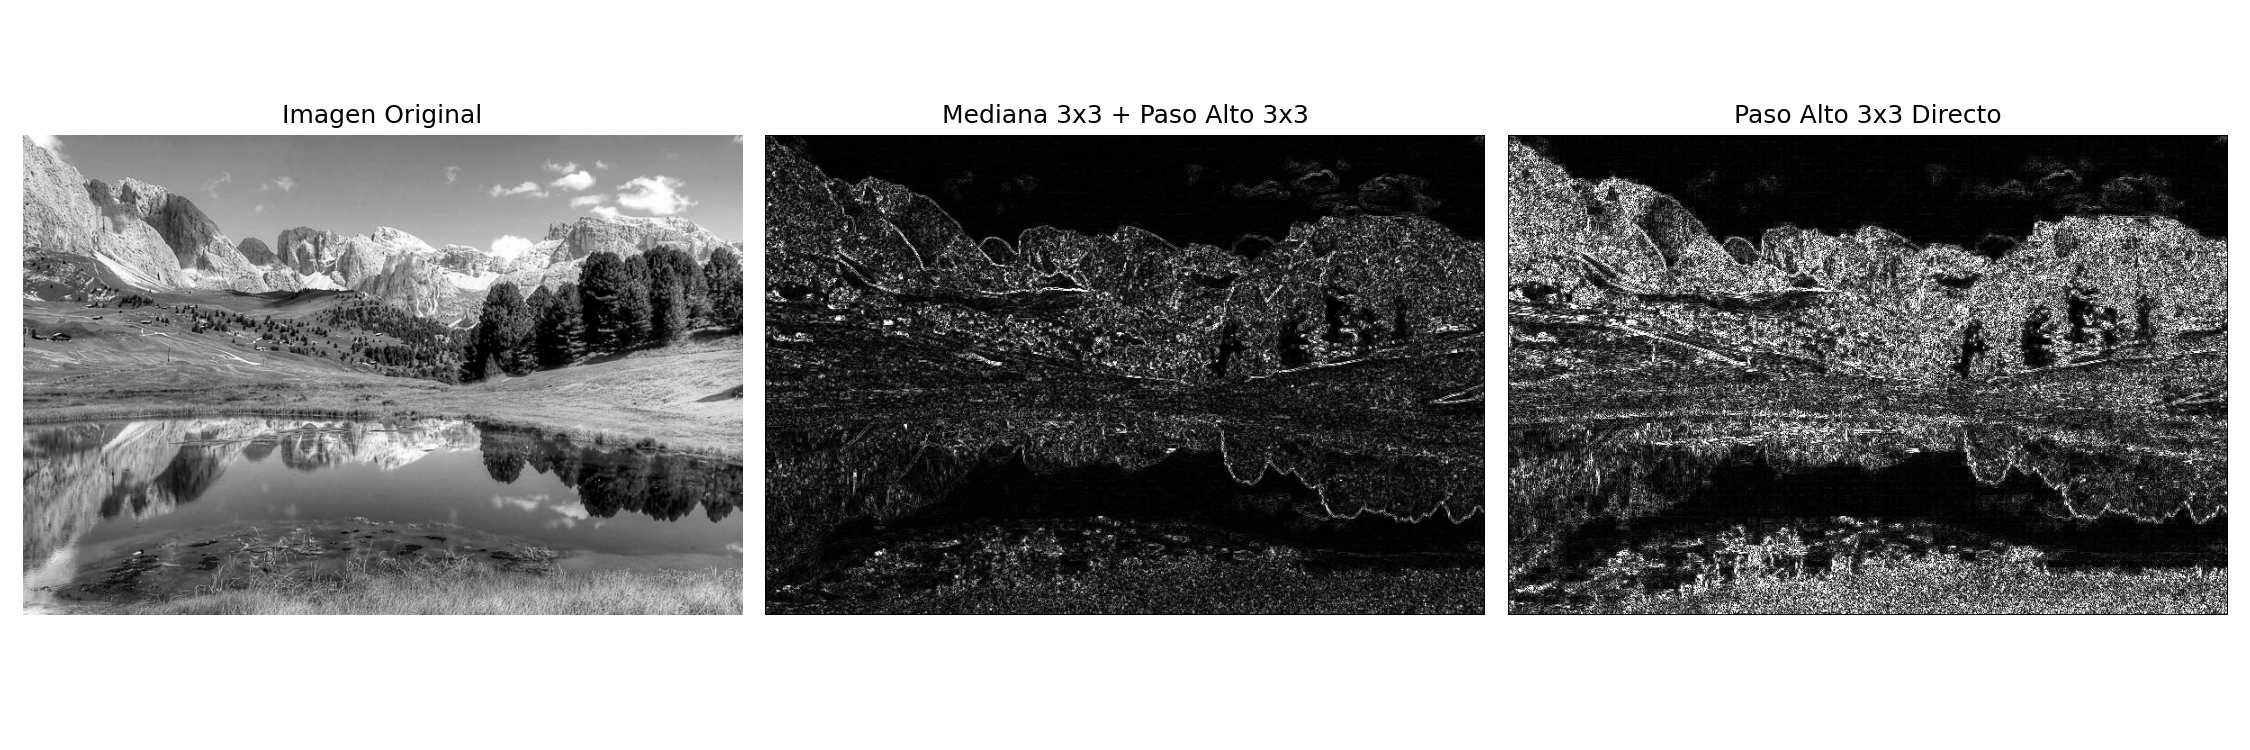
\includegraphics[width=\textwidth]
    {../results/resultado_mediana_paso_alto.png}
    \caption{Comparación entre el filtrado
    de mediana seguido de paso alto
    y la aplicación directa del paso alto.}
    \label{fig:combinado}
\end{figure}

\subsubsection*{Análisis de resultados}

Al observar las imágenes, se evidencia
que la combinación de mediana y paso alto
produce una imagen más oscura,
con menos detalles pequeños resaltados,
pero en la que se distinguen con mayor claridad
algunos bordes principales.

Esto se observa especialmente
en los contornos de las montañas,
los árboles y sus reflejos en el agua.

Por otra parte, al aplicar directamente
el filtro paso alto, se resaltan
muchas más variaciones de intensidad,
especialmente en la vegetación,
el pasto y las texturas de las montañas.

Esto genera una imagen con mayor
cantidad de puntos y regiones brillantes,
lo que dificulta distinguir algunos
de los contornos principales.

La diferencia se debe a que el filtro
de mediana reduce algunas variaciones
pequeñas de intensidad antes de aplicar
el filtro paso alto.

De esta manera, el paso alto posterior
resalta menos texturas y ciertos bordes
importantes pueden identificarse
visualmente con mayor facilidad.

Es importante aclarar que el filtro
de mediana no aumenta directamente
la intensidad de los bordes.

Su efecto consiste en reducir
parte de las variaciones locales,
permitiendo que algunos contornos
sobresalgan mejor respecto a su entorno.

En conclusión, aplicar primero
un filtro de mediana y después
uno paso alto permite reducir
detalles pequeños y mejorar visualmente
la identificación de ciertos bordes
principales.

Sin embargo, también puede eliminar
información fina de la imagen,
por lo que la elección del procedimiento
depende del objetivo del procesamiento.

% =========================================================
\section{Análisis general}

El desarrollo del taller permitió comprobar
que el filtrado espacial modifica
los valores de los píxeles teniendo
en cuenta la información de su vecindad.

En los primeros ejercicios se observó
que los filtros paso bajo producen
un efecto de suavizado.

El tamaño de la máscara y la distribución
de sus coeficientes influyen directamente
en la cantidad de detalles que se conservan.

La máscara ponderada $3\times3$ permitió
conservar mejor algunos bordes del paisaje,
mientras que las ventanas uniformes
más grandes produjeron un desenfoque mayor.

El filtro de media mostró que es posible
suavizar una imagen calculando directamente
el promedio de los valores vecinos.

Por su parte, el filtro de mediana
permitió aplicar una operación no lineal,
que reemplaza cada píxel por el valor
central de su vecindad ordenada.

En la fotografía utilizada,
la mediana produjo cambios relativamente
leves y conservó buena parte de los
contornos principales.

Posteriormente, los filtros paso alto
mostraron un comportamiento diferente:
en lugar de suavizar las variaciones
de intensidad, las destacaron.

Esto permitió identificar bordes
de montañas, árboles, vegetación
y reflejos sobre el agua.

También se observó que las máscaras
paso alto pueden producir respuestas
negativas o superiores a 255.

Los resultados del punto 4 demostraron
que una gran cantidad de píxeles
puede alcanzar el valor máximo
durante la visualización,
provocando saturación.

Finalmente, el punto 5 permitió
comprobar que combinar filtros
puede modificar significativamente
los resultados.

La aplicación previa de mediana
redujo algunas texturas y variaciones
pequeñas antes del filtro paso alto.

Como consecuencia, varios contornos
principales se distinguieron mejor
que en el resultado del filtrado
paso alto directo.

En conjunto, los ejercicios mostraron
que no existe un filtro universalmente
mejor, sino que su utilidad depende
de las características de la imagen
y del objetivo del procesamiento.

% =========================================================
\section{Conclusiones}

Los filtros espaciales permiten modificar
una imagen digital mediante operaciones
sobre los píxeles y sus vecinos.
Su implementación con ciclos facilitó
comprender el funcionamiento de las máscaras
y el cálculo de los nuevos valores.

Los filtros paso bajo de promedio y media
permitieron observar que una ventana
de mayor tamaño genera generalmente
un suavizado más intenso,
aunque también puede producir
una mayor pérdida de detalles.

El filtro de promedio ponderado
conservó mejor ciertos bordes
de la fotografía que el promedio uniforme
del mismo tamaño, debido a la mayor
importancia asignada al píxel central
y a sus vecinos cercanos.

El filtro de mediana permitió comprender
una forma diferente de procesar
la vecindad, utilizando el valor central
de una lista ordenada.
En las pruebas realizadas conservó
relativamente bien los contornos principales,
aunque también redujo algunos detalles finos.

Los filtros paso alto permitieron destacar
cambios bruscos de intensidad y visualizar
bordes y texturas presentes en el paisaje.

Además, se comprobó la importancia
de trabajar con tipos de datos adecuados,
ya que las operaciones pueden producir
valores negativos o superiores
al rango de una imagen de 8 bits.

La comparación final mostró que aplicar
un filtro de mediana antes del paso alto
reduce algunas variaciones pequeñas
y facilita la identificación visual
de ciertos bordes importantes.

En general, el taller permitió comprender
la relación entre
\textbf{máscaras, vecindad, suavizado,
mediana y detección de bordes},
así como la importancia de seleccionar
las técnicas de filtrado según
el resultado que se desea obtener.

\end{document}
